% !TeX spellcheck = it_IT
\section*{Introduzione}
\addcontentsline{toc}{section}{\protect\numberline{}Introduzione}
All'interno del corso sarà presente solo la progettazione di algoritmi, non si parla di architetture.\\

\paragraph{Contesto:} Generalmente parlando di algoritmi si considera un singolo esecutore, mentre con "paralleli e distribuiti" si aggiunge l'idea di avere una \textbf{pool di esecutori}, velocizzando possibilmente la risoluzione del problema, ma introducendo nuove problematiche. \\
Per un algoritmo non parallelo, quindi sequenziale, le \textbf{fasi} sono: 
\begin{itemize}
	\item \textbf{Progettazione:} scrittura dell'algoritmo, secondo diverse tecniche come \textit{divide et impera} (dividere il problema in sottoproblemi e combinare le sotto-soluzioni per la soluzione globale, es mergesort), \textit{programmazione dinamica} (utilizzare la memoria per memorizzare soluzioni parziali che saranno utilizzate per istanze più grandi, es calcolo Fibonacci), \textit{greedy} (per problemi di ottimizzazione, c'è una funzione da massimizzare/minimizzare, il problema generale viene risolto scegliendo a ogni passo la soluzione localmente ottima, migliore per quel singolo step, es algoritmo di Kruskal), ...
	
	\item \textbf{Valutazione delle prestazioni:} in termini di tempo, spazio di memoria e in generale valutare l'algoritmo nella sua complessità
	
	\item \textbf{Codificazione:} fase di implementazione con un opportuno linguaggio di programmazione
\end{itemize}

Per gli algoritmi paralleli le problematiche sono simili, ma l'unica tecnica che può essere riciclata è quella di divide et impera.  \\
Per gli algoritmi paralleli questi vengono valutati sempre in termini di tempo ma, al posto dello spazio, si conta il numero di processori. \\

Ma la pool di esecutori può avere diverse caratteristiche, ci sono due casi: 
\begin{itemize}
	\item \textbf{primo caso:} "una squadra in cui batte un solo cuore", più processori sincroni
	\item \textbf{secondo caso:} "ogni membro un mondo a parte", computer interfacciati ma ognuno ha il suo clock ed il suo tempo per risolvere le operazioni (es. diversi pc su internet), membri del pool lavorano in modo asincrono 
\end{itemize}


\subsection*{Primo caso: CPU Sincrone}
\addcontentsline{toc}{subsection}{\protect\numberline{}Primo caso: CPU Sincrone}
I processori sono sincroni, quindi vanno all'unisono, si ha un \textbf{clock centrale} che scandisce il tempo per l'intero insieme di processori quindi le \textbf{istruzioni vengono eseguite tutte assieme} in un tempo determinato per tutti.\\
Può essere che condividano risorse, come ad esempio una memoria comune, oppure i processori possono essere solo collegati tra loro .\\

Con la \textbf{memoria condivisa} il sistema si chiama \textbf{PRAM}, l'altro si chiama \textbf{sistema parallelo a memoria distribuita} (manca quella condivisa).\\

Esempio: 
\begin{center}
	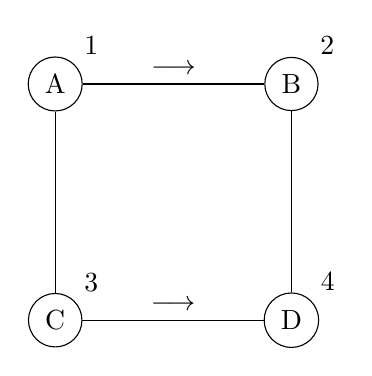
\begin{tikzpicture}
		\node[circle, draw, label=45:1] (A) at (0,0) {A};
		\node[circle, draw, label=45:2] (B) at (3,0) {B};
		\node[circle, draw, label=45:3] (C) at (0,-3) {C};
		\node[circle, draw, label=45:4] (D) at (3,-3) {D};
		
		\draw (A) -- (B) node[midway, above] {$\longrightarrow$};
		\draw (A) -- (C) node[below] {};
		\draw (D) -- (B) node[below] {};
		\draw (C) -- (D) node[midway, above] {$\longrightarrow$};
	\end{tikzpicture}
\end{center}

Memoria distribuita, ogni dato è in un processore diverso, i dati sono distribuiti. Generalmente i collegamenti sono full duplex (avanti e indietro, ambo le direzioni).\\

Operazioni: 

\begin{tabular}{c c}
	send(1,2) & send(3,4) \\
	A+B & C+D \\
	send(2,4) & \\
	A+B+C+D &
\end{tabular}

\newpage

Riga per riga: 
\begin{itemize}
	\item Il processore 1 invia A al 2, il 3 invia C al 4
	\item Nel processore 2 si fa la somma A+B, nel 4 si fa C+D
	\item Il processore 2 invia la somma al 4 
	\item Il 4 farà il totale.
\end{itemize}

Ogni riga permette un'operazione, si tratta di un ciclo di clock, quindi per fare questa somma in totale sono 4 cicli di clock. \\

In genere un solo processore contiene la risposta, solitamente quello con l'indice maggiore (ultimo, nel caso dei processori 1, 2, 3 e 4 il 4 contiene la risposta). \\

Con questo esempio non si capisce bene il guadagno dato dal parallelismo rispetto all'algoritmo sequenziale, ma si può generalizzare l'idea su un'istanza di lunghezza $n$, con un numero di processori adeguato (ma anche in caso di un numero di processori ridotti l'algoritmo si può adeguare alla situazione). In questo modo si può notare che il numero di passi scala in modo logaritmico con la dimensione $n$ (prima si sommano 2 a 2, poi 4 a 4, poi 8 a 8, ...). Si passa da $n$ passaggi con il sequenziale a $\log n$ con il parallelo. \\

\newpage

\subsection*{Secondo caso: CPU Asincrone}
\addcontentsline{toc}{subsection}{\protect\numberline{}Secondo caso: CPU Asincrone}
In questa casistica \textbf{ogni processore ha i propri tempi} nonostante siano \textbf{collegati tra loro}, e ovviamente non si può assumere memoria condivisa. Non avere un clock centrale porta ad avere algoritmi distribuiti e NON paralleli come nel caso precedente.\\
Non si può assumere \textbf{nessun tipo di sincronizzazione gratuita}, devono \textbf{scambiarsi dei messaggi} (es: attraverso internet, se non mi viene detto nulla non so niente degli altri processori).\\

Esempio: 
\begin{center}
	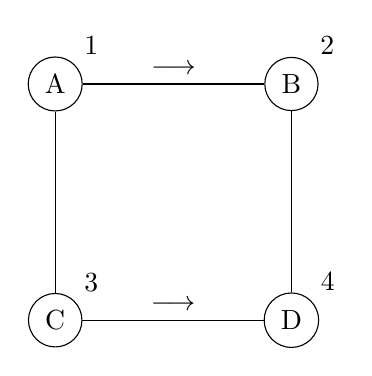
\begin{tikzpicture}
		\node[circle, draw, label=45:1] (A) at (0,0) {A};
		\node[circle, draw, label=45:2] (B) at (3,0) {B};
		\node[circle, draw, label=45:3] (C) at (0,-3) {C};
		\node[circle, draw, label=45:4] (D) at (3,-3) {D};
		
		\draw (A) -- (B) node[midway, above] {$\longrightarrow$};
		\draw (A) -- (C) node[below] {};
		\draw (D) -- (B) node[below] {};
		\draw (C) -- (D) node[midway, above] {$\longrightarrow$};
	\end{tikzpicture}
\end{center}

In questo caso potrebbero esserci \textbf{tempi} più lunghi e che \textbf{variano da collegamento a collegamento}, anche tra scambi diversi sullo stesso collegamento (come può accadere su internet). \\

Avendo velocità diverse, \textbf{un processore potrebbe dover aspettare} che gli altri terminino di elaborare/scambino i messaggi. \\
Serve scambiare messaggi per il coordinamento.\\

\newpage

\subsection*{Teoria e realtà: motivazioni}
\addcontentsline{toc}{subsection}{\protect\numberline{}Teoria e realtà: motivazioni}
Si studiano gli algoritmi a livello teorico, basandosi sulla realtà, esistono architetture distribuite per l'implementazione di tali algoritmi. La nascita di architetture parallele e distribuite comincia dalla seconda metà degli anni '60, di conseguenza si è sviluppata la teoria. \\

Esempi di architetture parallele: 
\begin{enumerate}
	\item \textbf{Supercomputer:} cluster di processori con incredibili prestazioni di calcolo (CDC, CRAY), solitamente a scopo di simulare sistemi complessi (fisici, militari, ...; tutto ciò che richiede un grande numero di operazioni aritmetiche). Di solito sono a memoria distribuita in quanto sarebbe difficile realizzarli a memoria condivisa dato che tutti i processori dovrebbero essere in grado di accedervi
	
	\item \textbf{GPU:} più processori collegati tra loro, in genere dedicate a problemi di grafica ma permettono di risolvere bene problemi di algebra lineare quindi viene usata in senso più generale
	
	\item \textbf{Multicore processor:} più unità di calcolo all'interno dello stesso processore, per migliorare le prestazioni ottimizzando l'assorbimento di energia (non bisogna aumentare il clock che porterebbe a un aumento dell'assorbimento) e relativi problemi di raffreddamento (meno energia meno calore); sistemi PRAM
	
	\item \textbf{Circuiti integrati:} sistemi di calcolo formati da gate opportunamente connessi; sostanzialmente una struttura a livelli che lavorano in parallelo prendendo input dal livello precedente
\end{enumerate}

Esempi di architetture distribuite:
\begin{enumerate}
	\item \textbf{Reti di calcolatori:} Internet (dagli anni '60), connettono dispositivi in molti diversi, quindi servono protocolli di comunicazione come TCP/IP
	
	\item \textbf{Reti mobili:} la topologia di connessione dei dispositivi cambia continuamente (gli smartphone si muovono)
	
	\item \textbf{Reti di sensori:} dispositivi con capacità limitate, per la maggior parte del tempo in "stand by", eseguono solo quello per cui sono costruite; solitamente hanno scopo di monitoraggio degli ambienti; necessitano di meccanismi di "wake up" (a un certo punto devo svegliarli), "acknowledge" (devono dire quando finiscono) e "recovery" (memorizzare le proprie informazioni/quelle ricevute)
\end{enumerate}

Negli \textbf{algoritmi paralleli} il fattore rilevante è il \textbf{tempo}. Nel sommare 4 numeri sono 4 passi, per sommarne 1000 ne servono 10. Per vedere se un algoritmo parallelo è efficiente si valuta il tempo. \\

Per gli \textbf{algoritmi distribuiti} quello che conta è il \textbf{coordinamento}, ovvero il \textbf{numero di messaggi da scambiare} (meno messaggi $=$ più veloce). Il numero di messaggi definisce una sorta di tempo e permette anche di avere un'idea della congestione della rete. \\

% End of L1

\subsection*{Problematiche parallele e distribuite}
\addcontentsline{toc}{subsection}{\protect\numberline{}Problematiche parallele e distribuite}

La \textbf{progettazione} richiede \textbf{nuove idee}, mentre la il processo di \textbf{valutazione} delle prestazioni richiede \textbf{nuove misure}.\\

\paragraph{Perché nuove idee?} Un algoritmo sequenziale efficiente non necessariamente porta a un algoritmo parallelo e/o distribuito efficiente, di conseguenza servono tecniche ad hoc per entrambi le tipologie.\\

Inoltre buoni algoritmi paralleli non sempre portano a buoni algoritmi distribuiti e viceversa. Ad esempio, nel \textbf{distribuito serve gestire problemi di ritardo e comunicazione}, che nel parallelo non si presentano.\\

Le misure che verranno definite non faranno riferimento a una architettura in particolare ma saranno definite solo in maniera teorica.\\

Per ogni paradigma si dovrà definire: 
\begin{enumerate}
	\item \textbf{Modello teorico}
	\item Come \textbf{valutare le performance} degli algoritmi
	\item \textbf{Semplici problemi} per apprendere le tecniche
\end{enumerate}

\newpage

Nel caso di \textbf{architetture parallele:}
\begin{enumerate}[label*=\Alph*.]
	\item Primo caso:
	\begin{enumerate}[label=\arabic*. ]
		\item \textbf{PRAM} (comunicazione immediata): memoria condivisa
		\item Risorse di calcolo: tempo, hardware (inteso come numero di processori)
		\item Problemi: sommatoria, somme prefisse, ordinamento
	\end{enumerate}
	\item Secondo caso
	\begin{enumerate}[label=\arabic*. ]
		\item Modello a \textbf{memoria distribuita}:
		\begin{itemize}
			\item array lineari: $n$ processori collegati all'interno di un array lineare, ovvero $P_i$ collegato a $P_{i+1}$, il quale è collegato a $P_{i+2}$ e così via
			\item mesh: versione bidimensionale dell'array lineare
			\item albero: albero binario completo di $n$ foglie
			\item ipercubo: per $n = 2^d$, un ipercubo (o $d$-cubo) è un grafo i cui vertici sono elementi $c_1, \, ... \, , c_d \in \{0,1\}^d$ e due vertici $x$ e $y$ sono estremi di un lato se le parole $x$ e $y$ differiscono in una sola posizione, quindi $P_x$ e $P_y$ sono collegati se $x$ e $y$ differiscono di una sola posizione. Sostanzialmente, un cubo ha $3$ dimensioni ed ogni vertice è collegato ad altri $3$, il $d$-cubo è la stessa cosa generalizzata in $d$ dimensioni, con un processore su ogni vertice. Inoltre è una struttura ricorsiva, un $d+1$-cubo è formato da $2$ $d$-cubi collegati tra loro, dove uno rappresenta la parte del $d+1$-cubo con bit più significativo a $0$, mentre l'altro la parte con bit più significativo ad $1$
		\end{itemize}
		\item Risorse di calcolo: tempo, hardware (processori non connessi direttamente comunicano più lentamente)
		\item Problemi: shuffle, max, ordinamento
	\end{enumerate}
\end{enumerate}

Nel caso di \textbf{architetture parallele:}
\begin{enumerate}
	\item Definizione del modello astratto 
	\item Risorse di calcolo: tempo, numero di messaggi (troppi $=$ congestione)
	\item Problemi: broadcast, wake up, traversal, spanning tree, election, routing
\end{enumerate}

\newpage

\subsection*{Il Tempo}
\addcontentsline{toc}{subsection}{\protect\numberline{}Il Tempo}

Gli algoritmi vanno \textbf{valutati} (anche) \textbf{sul tempo}, in quanto sia nel caso di algoritmi paralleli che di algoritmi distribuiti, la risorsa tempo è cruciale.\\

Come nel caso sequenziale, la \textbf{definizione formale} è:
\begin{itemize}
	\item $T(x) =$ numero di operazioni elementari su input $x$ (istanza). \\
	
	\item $t(n) = \max \{T(x) | \, x \in \Sigma^n \}$, il massimo valore di $T$tra tutti gli input di dimensione $n$, ovvero il caso peggiore tra tutte le istanze di dimensione $n$. Si tratta quindi di una funzione in $n$, dove $n$ è la dimensione dell'input.\\
\end{itemize}

Spesso non saremo interessati a una valutazione precisa ma a un \textbf{tasso di crescita della funzione}: quindi si usano le funzioni asintotiche $O, \Omega, \Theta$.\\

Definizioni (non formali, già viste troppe volte): siano $f,g: \mathbb{N} \rightarrow \mathbb{N}$ due funzioni definite sui numeri naturali
\begin{itemize}
	\item $f(n) = O(g(n))$, la funzione è limitata superiormente (da un certo punto in poi, non per forza da subito) dalla funzione $c \cdot g(n)$, per un valore di $c$
	
	\item $f(n) = \Omega (n)$, la funzione è limitata inferiormente (da un certo punto in poi) da $c \cdot g(n)$, per un valore di $c$
	
	\item $f(n) = \Theta(n)$, unione delle due sopra, limite stretto, ovvero la funzione è compresa tra $c_1 \cdot g(n) \leq f(n) \leq c_2 \cdot g(n)$
\end{itemize}
Tutte valgono asintoticamente, quindi da un certo punto in poi.\\

Da qui in poi sarà dato per scontato il concetto di MdT (chiamata Deterministic Turing Machine DTM), non lo riporterò, è già su almeno altri 2 blocchi di appunti e mi sono rotto il cazzo di scriverlo, comunque testina, quintupla, bla bla bla.\\

\newpage

\paragraph{Valutazione di $t(n)$:}
\begin{enumerate}
	\item Viene \textbf{valutata su} un particolare \textbf{modello di calcolo}, quando calcolo la funzione vado a contare il numero di operazioni
	\item Va scelto il \textbf{criterio di costo: uniforme o logaritmico}
\end{enumerate} 

Le \textbf{operazioni da contare} sono quelle \textbf{primitive messe a disposizione dal modello di calcolo}. \\
Esempio: palindromi
\begin{itemize}
	\item Input: $x \in \{0,1\}^\ast$
	\item Output: $x$ è palindroma
\end{itemize}
Soluzione: 
\begin{lstlisting}
	for(i=1, j=|x|; i<j && x_i = x_j; i++, j--);
	return i >= j;
\end{lstlisting}

Two pointers, controlla se ogni lettera è uguale a quella "dall'altro lato". Se si blocca (quindi non è palindroma) gli indici rimarranno tali che $i < j$ (e di conseguenza restituirà falso alla fine), altrimenti $i$ supererà $j$, dato che se arrivano a metà il controllo sarà valido fino alla fine portando gli indici a essere invertiti rispetto alla partenza.\\

Tale programma: 
\begin{itemize}
	\item su RAM (memoria ad accesso casuale) ha 
	$$ t(n) = O(n) $$
	(basta leggere una volta ogni lettera, posso accedere dove voglio nella memoria)
	\item Su DTM (una sola testina di lettura) ha 
	$$ t(n) = O(n^2) $$
	(devo fare avanti e indietro a ogni lettera che controllo)
\end{itemize}

\newpage

Inoltre bisogna \textbf{fare attenzione alla dimensione dei dati} in gioco. Esempio: Fattoriale
\begin{itemize}
	\item Input: $n \in \mathbb{N}$
	\item Output $n!$
\end{itemize}
Soluzione: 
\begin{lstlisting}
	k = 1; 
	for(i = 1; i <= x; k = k*i, i++);
	return k;
\end{lstlisting}
Effettua semplicemente il calcolo del fattoriale.\\

Tale programma:
\begin{itemize}
	\item Contando la moltiplicazione come operazione elementare di una RAM 
	$$ t(\log n) = n $$
	($\log n$ dato che $n$ è un numero naturale che si scrive in $\log n$ bit)
	\item su DTM, dovendo scrivere il binario il risultato $n! \simeq n^n$ abbiamo
	$$ t(\log n) \geq \log n^n = n \log n $$
\end{itemize}

\paragraph{Criteri di costo: }
\begin{itemize}
	\item \textbf{Uniforme:} le operazioni elementari richiedono una unità di tempo 
	\item \textbf{Logaritmico:} ogni operazione elementare ha un costo che dipende dal numero di bit degli operandi
\end{itemize}

\newpage

\subsection*{Teoria della Complessità}
\addcontentsline{toc}{subsection}{\protect\numberline{}Teoria della Complessità}

Possibili tassi di crescita di $t(n)$. Dobbiamo \textbf{stabilire quando qualcosa è efficiente per algoritmi paralleli e quando per i sequenziali}.\\

La funzione $t(n)$ si dirà: 
\begin{itemize}
	\item logaritmica quando è $O(\log n)$
	\item polilogaritmica quando è $O(\log^k n)$ per una costante $k>0$
	\item lineare quando è $O(n)$
	\item polinomiale quando è $O(n^k)$ per una costante $k>0$
	\item esponenziale quando NON è $O(n^k)$ per ogni costante $k>0$ 
\end{itemize}

\subsubsection*{Efficienza nel caso sequenziale}
\addcontentsline{toc}{subsection}{\protect\numberline{}Efficienza nel caso sequenziale}

Definizione formale: un problema è efficiente se ammette un \textbf{algoritmo efficiente}, ovvero viene \textbf{risolto} da una DTM in \textbf{tempo polinomiale}.\\

Si dicono:
\begin{itemize}
	\item $\mathcal{P} =$ classe dei problemi di decisione risolti in efficiente tempo
	\item $\mathcal{FP} =$ classe dei problemi generali risolti in efficiente tempo
\end{itemize}
Oppure
\begin{itemize}
	\item $\mathcal{P} =$ classe dei problemi di decisione risolti in tempo polinomiale
	\item $\mathcal{FP} =$ classe dei problemi generali risolti in tempo polinomiale
\end{itemize}

La differenza tra $\mathcal{P}$ e $\mathcal{FP}$ è che i problemi di decisione richiedono solo $sì$ o $no$, che sostanzialmente è il calcolo di un solo bit, mentre gli altri richiedono di calcolare più bit.\\

\newpage

Perché consideriamo il tempo polinomiale come efficiente? Esempio: considerando un processore da $4$ GHz ($\neq$ da una DTM) su un'istanza di 4000 caratteri (mezza pagina circa)
\begin{center}
	\begin{tabular}{c | c}
		complessità $t(n)$ & tempo di attesa \\
		\hline
		$n$ & $1\mu s$ \\
		$n^2$ & $4 ms$ \\
		$2^n$ & $> 1$ secolo \\
		$3^n$ & $\sim 2$ secoli e mezzo \\
	\end{tabular}
\end{center}


Come si può vedere i tempi esponenziali esplodono anche su istanze piccole.\\

Quindi: $\mathcal{P}$ e $\mathcal{FP}$ hanno una definizione robusta che non cambia con il modello di calcolo (non importa se sia su RAM o DTM).\\
Inoltre $\mathcal{P}$ e $\mathcal{FP}$ contengono molti problemi fondamentali, come ordinamento, prodotto di matrici, alcuni problemi di ottimizzazione, ...  \\

Purtroppo alcuni problemi interessanti non hanno ancora soluzioni efficiente e stanno in 
\begin{itemize}
	\item $\mathcal{NP} =$ problemi di decisione risolti in tempi polinomiale su una DTM non deterministica
\end{itemize}
Si congettura $\mathcal{P} \neq \mathcal{NP}$, ma non è ancora noto (non siamo certi che i problemi attualmente non risolvibili in tempo polinomiale non abbiano una soluzione efficiente).\\

I problemi che possono essere parallelizzati non possono appartenere ad $\mathcal{NP}$, altrimenti sarebbe come provare che $\mathcal{P} = \mathcal{NP}$.\\

All'atto pratico siamo interessati a una \textbf{sottoclasse di} $\mathcal{P}$
\begin{enumerate}
	\item La \textbf{valutazione asintotica} dei tempi può \textbf{nascondere costanti o termini} che all'atto pratico fanno la differenza. Esempio: a volte si preferisce il QuickSort ($O(n^2)$) rispetto al MergeSort ($O(n \log n)$).
	\item Da un punto di vista pratico il \textbf{grado del polinomio deve essere basso}. Es: $n^{1000}$ anche su piccole istanze risulta peggiore di un esponenziale. Esempio pratico: in $O(n^6)$ è il tempo per un test di primalità, ma il grado è troppo alto, quindi si preferisce un test probabilistico con possibilità di errore.
\end{enumerate}